\documentclass[12pt]{standalone}
\usepackage[T1]{fontenc}
\usepackage[utf8]{inputenc}
\usepackage{lmodern}

\usepackage{xcolor}
\usepackage{amsmath}
\usepackage{tikz}
\usetikzlibrary{3d,angles,quotes,calc}

\begin{document}
	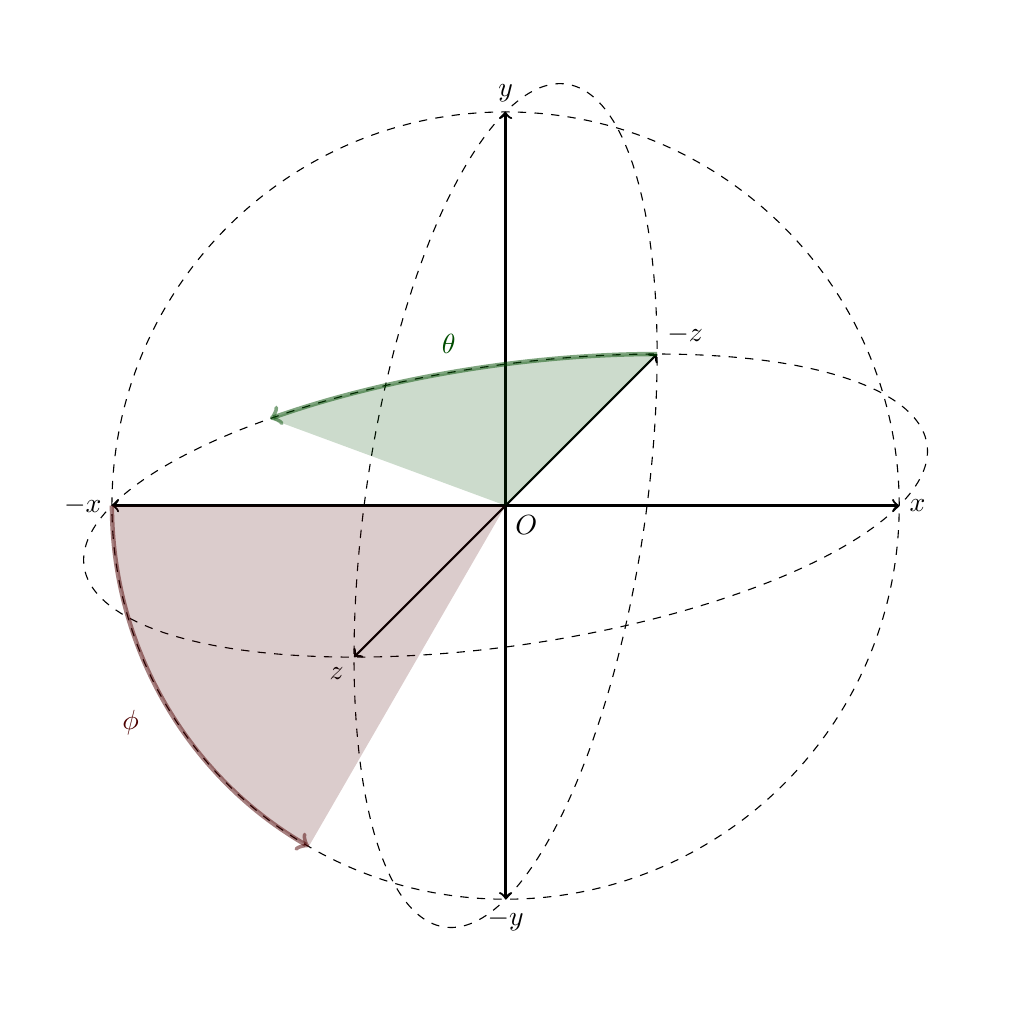
\begin{tikzpicture}[scale=5]
		\coordinate (O) at (0, 0, 0);
		\node[below right] at (O) {$O$};

		\begin{scope}[thick,->]
			\draw (O) -- (xyz spherical cs:radius=1,longitude=90) node[anchor=west]       {$x$};
			\draw (O) -- (xyz spherical cs:radius=1)              node[anchor=south]      {$y$};
			\draw (O) -- (xyz spherical cs:radius=1,latitude=90)  node[anchor=north east] {$z$};

			\draw (O) -- (xyz spherical cs:radius=1,longitude=-90)  node[anchor=east]       {$-x$};
			\draw (O) -- (xyz spherical cs:radius=1,longitude=180)  node[anchor=north]      {$-y$};
			\draw (O) -- (xyz spherical cs:radius=1,latitude=-90)   node[anchor=south west] {$-z$};
		\end{scope}

		\begin{scope}[dashed]
			\begin{scope}[canvas is yz plane at x=0]
				\draw (0, 0) circle (1);
			\end{scope}
			\begin{scope}[canvas is xz plane at y=0]
				\draw (0, 0) circle (1);
			\end{scope}
			\begin{scope}[canvas is xy plane at z=0]
				\draw (0, 0) circle (1);
			\end{scope}
		\end{scope}

		\begin{scope}[pics/angle/.append style={/tikz/transform shape,/tikz/pic text options={transform shape=false}}]
			\begin{scope}[canvas is xz plane at y=0,angle radius=10mm]
				\colorlet{colTheta}{green!30!black}
				\coordinate (theta0) at ({cos(-90)}, {sin(-90)});
				\coordinate (theta1) at ({cos(-145)}, {sin(-145)});
				\coordinate (O) at (0, 0);
				\draw pic[fill=colTheta,opacity=.2] {angle = theta1--O--theta0};
				\draw pic(theta)[draw=colTheta,"",ultra thick,<-,opacity=.5,angle eccentricity=1.2] {angle = theta1--O--theta0};
				\node at (theta) {\textcolor{colTheta}{$\theta$}};
			\end{scope}

			\begin{scope}[canvas is xy plane at z=0,angle radius=10mm]
				\colorlet{colPhi}{red!30!black}
				\coordinate (phi0) at ({cos(180)}, {sin(180)});
				\coordinate (phi1) at ({cos(240)}, {sin(240)});
				\coordinate (O) at (0, 0);
				\draw pic[fill=colPhi,opacity=.2] {angle = phi0--O--phi1};
				\draw pic(phi)[draw=colPhi,"",ultra thick,->,opacity=.5,angle eccentricity=1.1] {angle = phi0--O--phi1};
				\node at (phi) {\textcolor{colPhi}{$\phi$}};
			\end{scope}
		\end{scope}
	\end{tikzpicture}
\end{document}
